\documentclass[journal]{IEEEtran} % do not change this 

\usepackage{color}
%\usepackage{ulem}
\usepackage{amsmath,amsthm,amsfonts,amssymb,amscd}
\usepackage[pdftex]{graphicx}
\usepackage{graphicx}
\usepackage{multirow, booktabs}% to allow multiple-row elements in tabular environment
\usepackage[export]{adjustbox}
\usepackage{setspace}
\usepackage{rotating} % for landscape figure 


%\usepackage[toc,page]{appendix}
%%%%%%%%%%%%%%%%%%%%%%%%%%%%%%%%%%%%%%%%%%%%%%%%%%%%%%%%%%%%%%%%%%%%%%%%%%%%%
% users of pdfLaTeX must uncomment the following lines:
\usepackage{t1enc}% allows access to various special characters
%\usepackage{times}% change font to Nimbus Roman (based on Times Roman)
%%%%%%%%%%%%%%%%%%%%%%%%%%%%%%%%%%%%%%%%%%%%%%%%%%%%%%%%%%%%%%%%%%%%%%%%%%%%%


\usepackage{xspace}	% puts spaces after macros ONLY when needed (for example, before another word, but not before punctuation) 
\usepackage{hyperref} % helps with url formatting and auto-linking 

\usepackage{doi}
\usepackage[backend=bibtex,style=ieee,maxbibnames=9,maxcitenames=3]{biblatex}

\usepackage[table]{xcolor}
\usepackage{graphicx}
\usepackage{pdfpages}
\usepackage{hyperref}
\hypersetup{
    colorlinks=true,
    linkcolor=black,
    filecolor=magenta,      
    urlcolor=blue
}
\usepackage{steinmetz}
\setlength{\belowcaptionskip}{-10pt}
\usepackage{fullpage}
\usepackage{lastpage}
\usepackage{enumitem}
\usepackage{fancyhdr}
\usepackage{mathrsfs}
\usepackage{wrapfig}
\usepackage{setspace}
\usepackage{calc}
\usepackage{multicol}
\usepackage{cancel}
\usepackage[margin=2cm]{geometry}

% tikz packages
\usepackage{standalone}
\usepackage{tikz}
\usetikzlibrary{calc,positioning,matrix,shapes,patterns}
\usetikzlibrary{decorations.pathreplacing}
\newcommand\tikzmark[1]{
  \tikz[remember picture,overlay] \coordinate (#1);
}
\usepackage{pgfplots}
\pgfplotsset{compat=1.17} 
\usepgfplotslibrary{statistics}
% macros for formatting references within the document
\newcommand{\fref}[1]     {Fig.~\ref{#1}}
\newcommand{\tref}[1]     {Tab.~\ref{#1}}
\newcommand{\eref}[1]     {Equation~(\ref{#1})} % equation
\newcommand{\aref}[1]     {Alg.~\ref{#1}} % algorithm
\newcommand{\apref}[1]     {Appendix~\ref{#1}} % appendix
\newcommand{\sref}[1]     {Section~\ref{#1}} % section
\newcommand{\pref}[1]   {Part~\ref{#1}}
\newcommand{\trefs}[2] {Tables~\ref{#1} and~\ref{#2}}

% Text macros
\newcommand{\eg}    {\textit{e.g.}}
\newcommand{\ie}    {\textit{i.e.}}
\newcommand{\todo}[1]  {\textcolor{red}{TODO: #1}}
\newcommand{\quotes}[1]{`#1'}
\newcommand{\dquotes}[1]{``#1''}

%% Math formatting - these are used by later macros 
\newcommand{\xmath}[1]	{\ensuremath{#1}\xspace}% math with a space if needed
\newcommand{\bmath}[1]	{\xmath{\bm{#1}}}	% this is the best math bold!

%% Basic math commands
% fractions 
\newcommand{\onehalf}	{\xmath{\dfrac{1}{2}}}
\newcommand{\onehalft}{\xmath{\tfrac{1}{2}}} % 1/2 formatted for in-text
\newcommand{\onequarter}	{\xmath{\dfrac{1}{4}}}
\newcommand{\onethird}	{\xmath{\dfrac{1}{3}}}
\newcommand{\twothirds}	{\xmath{\dfrac{2}{3}}}
\newcommand{\paren}[1]{\xmath{\left(#1\right)}}

% operators 
\newcommand{\conv} 		{\circledast}  % convolution symbol
\newcommand{\abs}[1]   {\xmath{\lvert #1 \rvert}} % | . | absolute value 
\newcommand{\norm}[1]   {\xmath{\left\lVert#1\right\rVert}} % || . ||
\newcommand{\normsq}[1]   {\xmath{\left\lVert#1\right\rVert^2}} % || . ||^2
\newcommand{\normrsq}[1]{\xmath{\| #1 \|^2}} % "regular" - not big
\newcommand{\real}[1]{\;\xmath{\text{real} \left\{ #1 \right\}) }}
\newcommand{\sign}[1]{\xmath{\mathrm{sign}\left(#1\right)}}
\renewcommand{\log}[1] {\xmath{\operatorname{log}\mleft( #1 \mright)}} % trick to get proper spacing all around

% define other helpful math stuff 
\newcommand{\by}      {\xmath{\times}} % the x signal in a dimension, e.g., m x n 
\renewcommand{\neg}         {\xmath{\text{-}}} % this negative sign sometimes looks better than usting '-' in math mode

% Common part names
\newcommand{\R}[1]      {\xmath{R_{#1}}} % for example, \R{1} produces R_1 and \R{2} produces R_2
\newcommand{\C}[1]      {\xmath{C_{#1}}} 

% Common signal names 
\newcommand{\Vout}  {\xmath{V_\text{out}}}
\newcommand{\Vin}  {\xmath{V_\text{in}}}
\newcommand{\Vleft}  {\xmath{V_\text{left}}}
\newcommand{\Vright}  {\xmath{V_\text{right}}}



% helpful mathematical operators for electronics
\newcommand{\F}[1]{\xmath{\mathcal{F}\left\{#1\right\}}} % fancy F for Fourier transform
\renewcommand{\L}[1]{\xmath{\mathcal{L}\left\{#1\right\}}} % fancy L for Laplace transform % please add your own macros to this file! 
\addbibresource{references.bib}


\begin{document}

\title{Template for Electronics Final Project Report}


\author{Your name goes here% <-this % stops a space
\thanks{This is the final project report for ECE 2600 Electronics at the University of Virginia}}
% <-this % stops a space
%\thanks{J. Doe and J. Doe are with Anonymous University.}% <-this % stops a space
%\thanks{Manuscript received April 19, 2005; revised August 26, 2015.}}


\maketitle

%%%%%%%%%%%%%%%%%%%%%%%%%%%%%%%%%%%%%%%%%%%%%%%%%%%%%
\section{Key project report requirements}

\todo{Delete this section before finalizing your report.}

Latex and Overleaf work through writing code and compiling it.  
You will write your text in the left hand plane, then click the green 'Recompile' button to see the changes in the pdf on the right.  
One thing to get used to is that a new line in the code does not automatically yield a new paragraph.  
To get a new paragraph, you need to hit enter twice and have a blank line between text. 
This becomes useful when you want to add things like bullets and equations in line.
There is a wealth of online help on how to write code in latex, so if you don't know how to do something try googling it or ask us--we're more than happy to help with Latex questions. 


Throughout the report, cite any references that you used. 
To do so, use the cite command and add the reference in the references.bib file. 
An example citation is \cite{tle2426}.
You can also have an in-text citation using the `textcite' command, \eg, \textcite{fung:2022:jfbjacobianfreebackpropagation}.
You should minimally include citations for the AD2 \cite{AD2} and Multisim \cite{Multisim} or KiCad \cite{KiCad} the first time you reference them. 

Here is an example equation for a voltage divider
\begin{equation}
    \Vout = \frac{R_1}{R_1 + R_2} \Vin 
    \label{eq: resistor divider}
.\end{equation}
Notice that the equation is part of a sentence and is punctuated as such. 
You can reference an equation using the eref macro, \eg, \eref{eq: resistor divider} is the voltage divider equation. 
Equations can also be written in line using dollar signs, \eg, 
\begin{verbatim}
    $X+Y=5$
\end{verbatim}
renders as $X+Y=5$.
This works well for simpler equations, but if you start to have large fractions or other complex equations, it is better to do them on their own line in an equation or align environment. 
This link has details on writing equations in latex: \url{https://www.overleaf.com/learn/latex/mathematical_expressions}. 

 
Use the 'enumerate' command to make numbered lists:
\begin{enumerate}
  \item First bullet.
  \item This is my second bullet.
\end{enumerate}

Upload figures as images in the file navigator toolbar on the left.  
You can reference figures using the fref command.
For example, \fref{fig: full schematic} shows a schematic of the audio analyzer. 
You should reference this figure in your report. 
Do not overwhelm your report with excess figures--%
include only figures that add to your report.



\begin{sidewaysfigure*}
    \caption{\todo{All captions should be sentences in normal sentence case (do not capitalize every word). Tell the reader why the figure is here and what they should take away from it.}}
    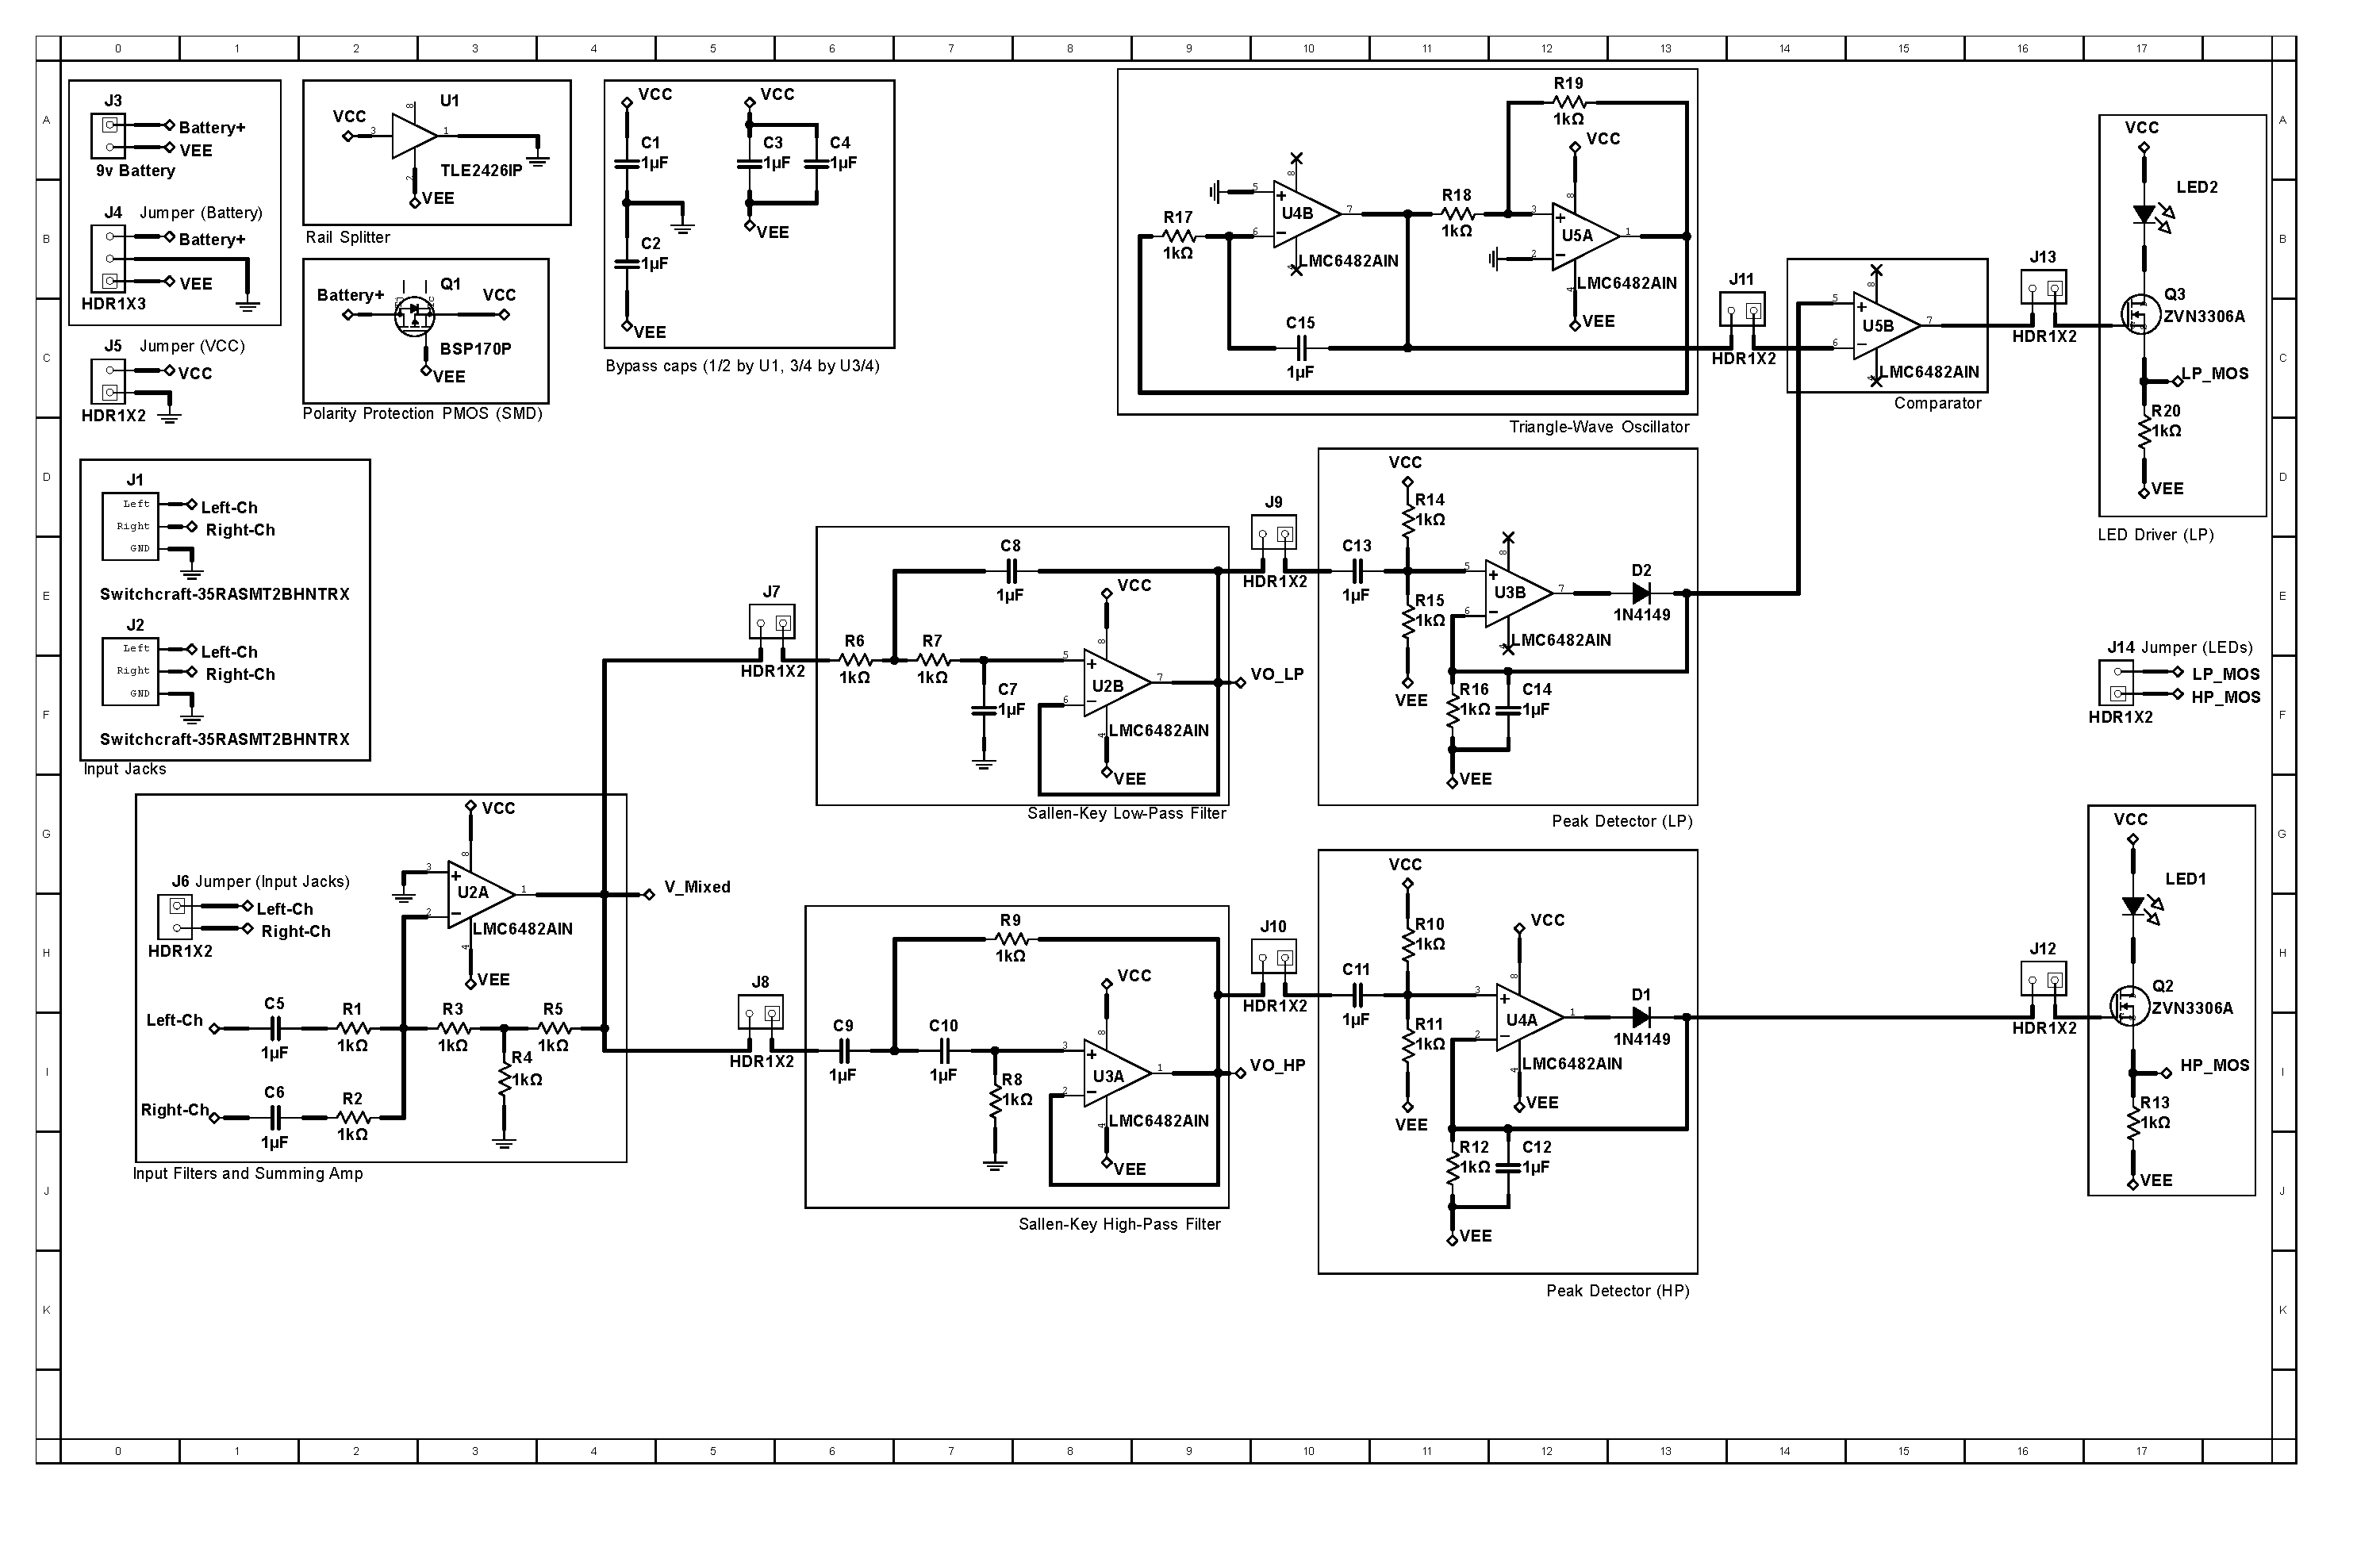
\includegraphics[width=\textwidth]{images/AudioAnalyzer_Schematic.pdf}
    \label{fig: full schematic}
\end{sidewaysfigure*}

%%%%%%%%%%%%%%%%%%%%%%%%%%%%%%%%%%%%%%%%%%%%%%%%%%%%%%%%%%%%%%%%%%%%%%%%%%%%%%%%
\section{High and Low Pass Filters}
\todo{Add a short paragraph to situate the reader to the purpose of this sub-system in the overall project.
This intro should be high-level. 
It should not have any equations or variables.
See the peak detector activity for an example.}

\subsection{Design and Analysis}
\todo{Write about design and analysis of the HPF and LPF here.}


This section should minimally include 
\begin{enumerate}
    \item parametric equations describing how the filters work in terms of the component designators from the project schematic with a reference to the TI document \cite{sallen_key} and a brief explanation for any differences from the equations in \cite{sallen_key}, 
    \item a description of how you came up with the designed values, typically written in terms of the provided requirements and any additional design goals, as applicable, and
    \item the resulting expected performance (corner frequency and quality factor). 
\end{enumerate}
Make sure to define all variables that you use. 
You do not need to include your own schematic nor update \fref{fig: full schematic} when you turn in this sub-section. 

\subsection{Simulation and Experimental Results}
\todo{Show your simulations of the HPF and LPF here.}
Make sure to include measurement setup, such as input settings, as well as the results themselves. 
Consider what results you need to include to convince the reader that your design works. 
Include 1-2 well-formatted graph(s) showing how you verified the design. 

Any time you are presenting results, clearly explain what the reader should take away from the results.
Why did you include the result? What does it prove? 
Do not present data without any story or interpretation.

A challenge with technical writing is to be concise (don't include excess information) \textit{and} precise (include sufficient information). 


%%%%%%%%%%%%%%%%%%%%%%%%%%%%%%%%%%%%%%%%%%%%%%%%%%%%%%%%%%%%%%%%%%%%%%%%%%%%%%%%


%%%%%%%%%%%%%%%%%%%%%%%%%%%%%%%%%%%%%%%%%%%%%%%%%%%%%%%%%%%%%%%%%%%%%%%%%%%%%%%%
\begin{singlespace}
\printbibliography
\end{singlespace}

\end{document}
